\PassOptionsToPackage{unicode=true}{hyperref} % options for packages loaded elsewhere
\PassOptionsToPackage{hyphens}{url}
%
\documentclass[12pt,]{article}
\usepackage{lmodern}
\usepackage{amssymb,amsmath}
\usepackage{ifxetex,ifluatex}
\usepackage{fixltx2e} % provides \textsubscript
\ifnum 0\ifxetex 1\fi\ifluatex 1\fi=0 % if pdftex
  \usepackage[T1]{fontenc}
  \usepackage[utf8]{inputenc}
  \usepackage{textcomp} % provides euro and other symbols
\else % if luatex or xelatex
  \usepackage{unicode-math}
  \defaultfontfeatures{Ligatures=TeX,Scale=MatchLowercase}
    \setmainfont[]{Times New Roman}
\fi
% use upquote if available, for straight quotes in verbatim environments
\IfFileExists{upquote.sty}{\usepackage{upquote}}{}
% use microtype if available
\IfFileExists{microtype.sty}{%
\usepackage[]{microtype}
\UseMicrotypeSet[protrusion]{basicmath} % disable protrusion for tt fonts
}{}
\IfFileExists{parskip.sty}{%
\usepackage{parskip}
}{% else
\setlength{\parindent}{0pt}
\setlength{\parskip}{6pt plus 2pt minus 1pt}
}
\usepackage{hyperref}
\hypersetup{
            pdftitle={Analyzing Forest Elephant Trails in Gabon, Africa},
            pdfauthor={Elise Harrigan and Katie Krejsa},
            pdfborder={0 0 0},
            breaklinks=true}
\urlstyle{same}  % don't use monospace font for urls
\usepackage[margin=2.54cm]{geometry}
\usepackage{longtable,booktabs}
% Fix footnotes in tables (requires footnote package)
\IfFileExists{footnote.sty}{\usepackage{footnote}\makesavenoteenv{longtable}}{}
\usepackage{graphicx,grffile}
\makeatletter
\def\maxwidth{\ifdim\Gin@nat@width>\linewidth\linewidth\else\Gin@nat@width\fi}
\def\maxheight{\ifdim\Gin@nat@height>\textheight\textheight\else\Gin@nat@height\fi}
\makeatother
% Scale images if necessary, so that they will not overflow the page
% margins by default, and it is still possible to overwrite the defaults
% using explicit options in \includegraphics[width, height, ...]{}
\setkeys{Gin}{width=\maxwidth,height=\maxheight,keepaspectratio}
\setlength{\emergencystretch}{3em}  % prevent overfull lines
\providecommand{\tightlist}{%
  \setlength{\itemsep}{0pt}\setlength{\parskip}{0pt}}
\setcounter{secnumdepth}{5}
% Redefines (sub)paragraphs to behave more like sections
\ifx\paragraph\undefined\else
\let\oldparagraph\paragraph
\renewcommand{\paragraph}[1]{\oldparagraph{#1}\mbox{}}
\fi
\ifx\subparagraph\undefined\else
\let\oldsubparagraph\subparagraph
\renewcommand{\subparagraph}[1]{\oldsubparagraph{#1}\mbox{}}
\fi

% set default figure placement to htbp
\makeatletter
\def\fps@figure{htbp}
\makeatother

\usepackage{etoolbox}
\makeatletter
\providecommand{\subtitle}[1]{% add subtitle to \maketitle
  \apptocmd{\@title}{\par {\large #1 \par}}{}{}
}
\makeatother

\title{Analyzing Forest Elephant Trails in Gabon, Africa}
\providecommand{\subtitle}[1]{}
\subtitle{\url{https://github.com/kmk85/HarriganKrejsa_ENV872_EDA_FinalProject}}
\author{Elise Harrigan and Katie Krejsa}
\date{}

\begin{document}
\maketitle

\newpage
\tableofcontents 
\newpage
\listoffigures 
\newpage

\hypertarget{rationale-and-research-questions}{%
\section{Rationale and Research
Questions}\label{rationale-and-research-questions}}

\hypertarget{elephant-movement-in-gabon-africa}{%
\subsection{Elephant Movement in Gabon,
Africa}\label{elephant-movement-in-gabon-africa}}

Elephants are universally some of the most beloved and threatened
species in Africa. As a charismatic megafauna, they capture the
attention of people as a majestic and powerful animal roaming the
African forest and plains. But elephants are also critical in forest
ecosystems. As elephant herds travel, they remove trees to create space,
consume an incredible amounts of vegetation and use water bodies and
dirt piles to cool off. The daily actions of elephants inevitably leave
a network of trails in their wake. To be able to better understand
forest elephants' daily movements, we will study the trails used by the
forest elephant of Gabon.

Gabon is a country located on the western coast of Africa and covered in
dense forest. Due to the forest canopy coverage, collecting data on the
elephant trails can be difficult because satellite imagery is not able
to penetrate past the top layers of the forest to capture the trail
locations on the forest floor. In order to gather more information on
elephant movements, data were collected in the field and was analyzed in
this study.

\hypertarget{study-questions}{%
\subsection{Study Questions}\label{study-questions}}

This study focused on understanding the use of elephant trails and the
frequency of travel on these trails. We analyzed the condition of trail
as poor, medium or heavy trodden, the width of the trail, and the use
denoted by the start, stop or change direction in the trail. We aimed to
answer the following questions to gain information on the activity level
of elephants and the use of the trails.

\begin{enumerate}
\def\labelenumi{\arabic{enumi}.}
\tightlist
\item
  What is frequency and number of days traveled on each trail?
\item
  What is the condition and use of the trail?
\end{enumerate}

By studying and better understanding the movements and patterns of
elephants, future researchers will be able to compare how elephants
react to human disturbance, how they impact the vegetation, and their
patterns across the landscape.

\newpage

\hypertarget{dataset-information}{%
\section{Dataset Information}\label{dataset-information}}

The data used for this project were collected in and around Ivindo
National Park, Gabon by a team of Duke University researchers, local
field guides, and forest peoples. Two datasets were provided to us by Dr
Amelia Meier of Duke University. Data for waypoints and tracklogs were
collected in the field with GPS units as the team searched for and
walked along forest elephant trails. The data are both spatial,
containing geographic coordinates, and temporal, containing date and
time components.

The tracklogs dataset includes GPS data where the field teams were
walking. Data contained in this dataset includes the site name (Ivindo),
date, time, latitude, and longitude, where everything is recorded in
decimal degrees WGS84. The dates of the tracklogs range from February
2018 to May 2018.

The waypoints dataset includes the waypoints taken by field teams when
they started walking on an elephant trail or if the elephant trail
changed characteristics. The data contained in this dataset includes
date, time, latitude, longitude, trail characteristics (cmt), data on
where the elephant trails started and stopped and when the field team
got on or of a trail (name), and the symbol used in the GPS (sym). More
specifically, the ``name'' field includes ``start'' or ``stop'' if the
team got on or off a trail, ``trstart'' or ``trstop'' if the trail
itself started or disappeared, ``change'' if a characteristic of the
trail change, and ``jct'' if they came to a trail crossing. In the cmt
field, there are two sets of information: a letter (P = poor, M =
medium, H = heavy) representing how heavily trodden the path is and a
number representing the width of the trail in cm. If the cmt section is
blank then the details previously recorded remained the same. Data
contained in this dataset was also recorded in decimal degrees WGS84 and
the dates of data collection also range from February 2018 to May 2018.

\begin{longtable}[]{@{}llll@{}}
\toprule
\textbf{Dataset} & \textbf{Variables} & \textbf{Range or Unique Values}
& \textbf{Central Tendancies}\tabularnewline
\midrule
\endhead
IV\_tracklogs & site & & -\tabularnewline
- & time & &\tabularnewline
- & latitude & -0.3429768 - 0.6005945 & mean = 0.07083619; median =
-0.1230693\tabularnewline
- & longitude & 12.43589 - 12.81332 & mean = 12.60479; median =
12.60231\tabularnewline
IV\_wgts & date & 2018-02-06 - 2018-05-25 &\tabularnewline
- & time & &\tabularnewline
- & latitude & -0.335521 - 0.599461 & mean = 0.2283088; median =
0.486579\tabularnewline
- & longitude & 12.43817 - 12.80200 & mean = 12.66357; median =
12.72618\tabularnewline
- & name & &\tabularnewline
- & sym & &\tabularnewline
- & cmt (letter) & ``P'' ``M'' ``W'' &\tabularnewline
- & cmt (number) & 35 - 75 & mean = 50; median = 47.5\tabularnewline
\bottomrule
\end{longtable}

\hypertarget{data-wrangling}{%
\subsection{Data Wrangling}\label{data-wrangling}}

The overall goal in wrangling our data was to combine the two files so
that all the points on the tracklogs are assigned trail characteristics
(on trail, off trail, size and use of trails). Doing this would then
allow us to quantify the types of trails that elephants use in which
contexts.

The tracklogs dataset included a total of 76,098 observations of 6
variables (X, site, date, time, lat, and lon), and the waypoints dataset
included a total of 452 observations of 8 variables (X, date, time, lat,
lon, name, sym, and cmt). To assign trail characteristics (cmt and name)
from the waypoints dataset to the tracklogs dataset, we could not do a
simple join because the dates and times did not match up exactly. So
instead, we first identified all of the unique dates in the waypoints
dataset. We then filtered the tracklogs dataset so that it only included
the unique dates found in the waypoints dataset. This reduced the number
of tracklog observations to 42,179.

Because there are many observations on each day, we next combined the
date and time columns to create a combined date\_time column in each of
the two datasets and arranged both datasets by ascending order of
date\_time. As stated earlier, the two datasets do not have exact
matching date\_time entires, so to assign cmt column values to the
tracklogs dataset based on date\_time, we transferred cmt values to the
tracklogs dataset if the tracklogs date\_time was within a window of the
date\_time column of the waypoints dataset using a for loop. We then
filtered out all of the ``NA'' values of the resulting tracklogs
dataset. We were told that if the ``cmt'' column is blank then the
details previously recorded remained the same; Therefore, we filled in
blanks with previously recorded values by first filling cells of empty
strings with ``NA'' and then using the fill() command. Because the cmt
column holds two pieces of information (a letter representing how
heavily trodden the path is and a number representing the width of the
trail), we separated these into two separate columns using the
str\_extract() command. Last, we assigned the ``name'' column values to
the tracklogs dataset in the same way as we assigned the cmt values,
using a for loop.

\newpage

\hypertarget{exploratory-analysis}{%
\section{Exploratory Analysis}\label{exploratory-analysis}}

The elephant trail dataset has dimensions of 40,910 observation and 11
variables. We looked primarily at the use and the width of each trail
and the longitude and latitude. First, we wanted to see the total amount
of trails for each use type (P, M, W) in order to see which type of
trail was most common. By summarizing the total amounts of each use of
trail, we were able to see the Poor trails were the most commonly
described trail.

\begin{longtable}[]{@{}ll@{}}
\toprule
\textbf{Use of Trail } & \textbf{Total Amount}\tabularnewline
\midrule
\endhead
Poor (P) & 27,218\tabularnewline
Medium (M) & 13,666\tabularnewline
Heavy (W) & 26\tabularnewline
\bottomrule
\end{longtable}

Visualizing these trails was also helpful to explore these data
spatially. To do this, we used mapview to get an idea of where the
trails are located and the type of condition the elephants were
traveling on. Given the size of the dataset, we created a subset to just
look at one date where all three trail types were present. On April 15,
2018, all three trails were documented which made this a good date to
further examine.

The map shows how the elephants traveled with each point representing a
location captured. Here you can also see the majority of the trails are
considered poorly trodden until the trails begin to congregate, and we
see an increase in the number of medium and heavily trodden trails.
Further investigation could occur using remote sensing techniques such
as lidar, which would allow us to see if there is a environmental
feature such as a water body, bringing the elephants to this area.

\begin{verbatim}
## PhantomJS not found. You can install it with webshot::install_phantomjs(). If it is installed, please make sure the phantomjs executable can be found via the PATH variable.
\end{verbatim}

\newpage

\hypertarget{analysis}{%
\section{Analysis}\label{analysis}}

A research questions for this study were to gain information on how many
trails were occurring each day, the type of condition of the trails and
if the width of the trail was statistically significant to the type of
use. To address the first part of this question, we took a deeper dive
into analyzing how many trails were occurring for each day by examining
the relationship between the days and the number of trails for each day.

\begin{figure}

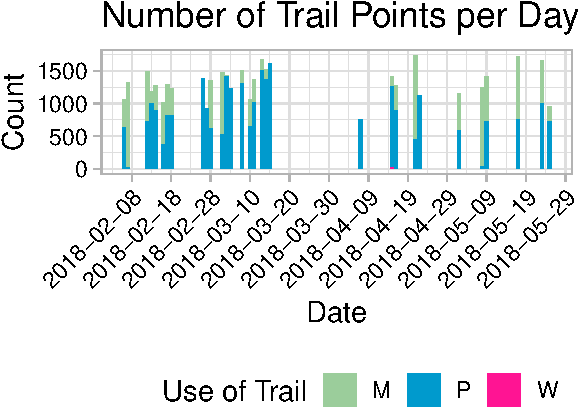
\includegraphics{Project_Template_files/figure-latex/unnamed-chunk-2-1} \hfill{}

\caption{The poor trodden trails are more abundant earlier in the year and the medium trodden trails take over in late April-May timeframe.}\label{fig:unnamed-chunk-2}
\end{figure}

For the second part of our research question, we analyzed the widths and
condition of each trail by graphing the relationships. It was evident
that the heavy trails also had the greatest width and the poor and
medium trails had relatively similar widths.

To test our assumptions about the significance of the width of trail to
the type, we performed a statistical analysis using a linear regression.
We ran a post-hoc Tukey test to determine if the different levels of
trail use are statistically different from each other.

\begin{figure}

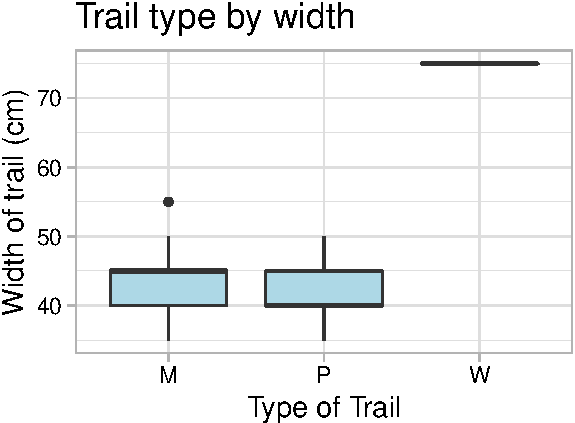
\includegraphics{Project_Template_files/figure-latex/plots by width-1} \hfill{}

\caption{On the x axis, the three letters represent how heavily trodden the path is:  (P = poor, M = medium, W = heavy) and the width of the trail on the y-axis in centimeters.}\label{fig:plots by width}
\end{figure}

\begin{figure}

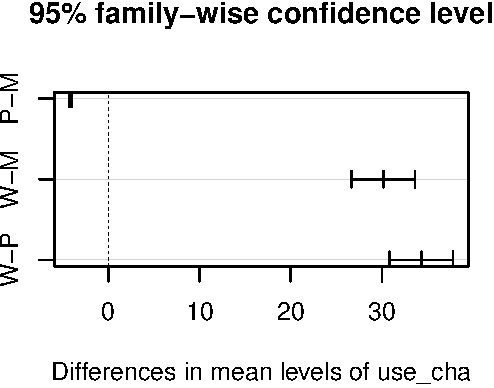
\includegraphics{Project_Template_files/figure-latex/unnamed-chunk-3-1} \hfill{}

\caption{Post-hoc Tukey test for trail use.}\label{fig:unnamed-chunk-3}
\end{figure}

\newpage

\hypertarget{summary-and-conclusions}{%
\section{Summary and Conclusions}\label{summary-and-conclusions}}

The first question we wanted to answer was to see the number of trail
points occurring for each day. In general, you can see that the level of
use increased from poorly trodden to medium trodden over time. By
looking at the graph, the poor trodden trails are more abundant earlier
in the year and the medium trodden trails become more abundant in April
and May.

In our final dataset, which included only the data that were recorded on
common dates between our two initial datasets, there are 27,218 poor
trodden trail points, 13,666 medium trodden trail points, and 26 heavily
trodden trail points. From our analyses on the widths of each type of
trail, we found that the heavily trodden trail is significantly wider
than the poor and medium trodden trails and the widths of the poor and
medium trodden trails are not significantly different. While the heavily
trodden trails are significantly wider than the poor and medium trodden
trails, it is important to note that the heavily trodden trails have a
much smaller number of recorded trail points, which occur in a compact
geographic area compared to all of the other recorded points, and only
on one day. Overall, we can conclude that the majority of recorded trail
points are poorly trodden (67\%) and medium trodden (33\%), and very few
are heavily trodden (\textless{}0.1\%).

The preliminary analyses presented in this project, provide an initial
exploration into the uses for these data. In future studies, these data
could be used to see how the trails change due to human disturbance or
presence, or to see how and where elephants do or do not change course.
There are also opportunities with these data to look at the change of
vegetation along the different use trails and if it will affect the
reproduction, seed dispersal or the types of plants that come up in the
forest gaps.

\end{document}
